%!TEX root = ../thesis.tex
%*******************************************************************************
%****************************** Third Chapter **********************************
%*******************************************************************************
\chapter{Quantifying and classifying tissue structure}

% **************************** Define Graphics Path **************************
\ifpdf
    \graphicspath{{Chapter3/Figs/Raster/}{Chapter3/Figs/PDF/}{Chapter3/Figs/}}
\else
    \graphicspath{{Chapter3/Figs/Vector/}{Chapter3/Figs/}}
\fi
\section{Introduction}
As shown in the previous section, stromal and epithelial immune infiltration may have differing roles within the response to a developing tumour. It is clear from observing image of tumour sections that the structure of the epithelium and stromal regions varies dramatically. These morphological differences have been discussed by Lisio et al. \cite{Lisio2019Feb} amongst others. This section of the thesis aims to set out an automated classification of such tissue structure, to investigate whether this can be reliably obtained from multiple types of tissue image and whether the structure defined this way is related to the infiltration of the tumour by particular types of immune infiltrate.  The workflow of this Chapter is illustrated in Figures \ref{fig:VA_ch4} and \ref{fig:VA_ch4_2}.

\begin{figure}
    \centering
    \includegraphics{Chapter3/Figs/Chapter3_VA.PNG}
    \caption{Visual Abstract for Chapter 4}
    \label{fig:VA_ch4}
\end{figure}

\begin{figure}
    \centering
    \includegraphics{Chapter3/Figs/VAch2_2.png}
    \caption{Visual Abstract for Chapter 4}
    \label{fig:VA_ch4_2}
\end{figure}

\section{Collaborators and Roles}
Sarwah Al-Khalidi(SAK) stained the OV04 TMA sections for CK7 and H\&E.

\section{Methodology}
\subsection{Patient Cohorts}
Data from the OV04 Cohort was used for this section as it had existing sections that had H\&E and CK staining. This cohort also had sections available for further analysis using SHG. 

\subsection{IHC}
\subsubsection{Cytokeratin 7 staining}
Tissue sections from the OV04 cohort were stained with Cytokeratin7 by Sarwah Al-Khalidi and the method of staining and imaging is laid out in section \ref{sec:sarwah_staining}.

\subsection{H\&E}
Automated Haemotoxylin and Eosin staining was carried out by SAK and is described in \ref{sec:sarwah_staining}. 

\subsection{SHG}
SHG microscopy excited at wavelength 900nm and detected at 440-460nm was performed on the Leica SP5 microscope and imaged using a 20x objective. DAKO mounting media and a coverslip of thickness 150$\mu$m was used. 

\subsection{DBSCAN}
The package \textbf{dbscan} in R was used for density based clustering analysis. The mathematics of this method is discussed in the Methods. 

\section{Results}
Having found in the previous chapter that the specific localisation of several immune infiltrates was an important factor in the prognosis of patients, I wanted to investigate the structure of tissue sections and assess the impact of structure on immune infiltrate. I wanted to use both H\&E and Cytokeratin stained images to derive this structure. Cytokeratin 7 was used as an epithelial marker to have a gold standard for structure analysis and to validate tissue classification of H\&E so that structures can be compared across multiple sections from the same core.

The morphologies discussed by Lisio et al are solid architecture, glandular architecture with slit-like spaces, papillary architecture and cribriform and pseudoendometroid architecture\cite{Lisio2019Feb} and in order to assess whether these structures could be automatically derived from images, the segmentation of tumour and stroma cells must first be acquired. 

\subsection{Patient Characteristics}
TMAs had been previously constructed from the CTCR-OV04 clinical studies, which were designed to collect imaging, blood, and tissue samples for exploratory biomarker studies. All patients provided written, informed consent for participation in these studies and for the use of their donated tissue, blood specimens, and anonymized data for the laboratory studies carried out. The CTCR-OV04 studies were approved by the Suffolk Local Research Ethics Committee (reference 05/Q0102/160) and Cambridgeshire Research Ethics Committee (reference 08/H0306/61).\cite{}

This cohort contained 40 patients with HGSOC. Samples were collected where possible for each patient from Normal Fallopian Tube, Malignant Ovary, Omentum and Metastasis. Two cores were extracted per tissue block where possible and two TMA blocks were constructed per tissue type.

\begin{table}[]
    \centering
    \begin{tabular}{lc}
    \hline
       N  &  40 \\
        Age &  77 (60-90)
    \hline
    \end{tabular}
    \caption{OV04 study patient characteristics}
    \label{tab:OV04_patient}
\end{table}


\subsection{Cell classifier performance and comparison between H\&E and CK}

Images of tissue sections stained with both H\&E and a CK7 marker were analysed. QuPath was used to segment nuclei based upon their optical density. Nuclei were then classified based upon size, shape and smoothed features using a random forest based classifier. Cells were split randomly into a test and training data set. Examples of tissue classification on H\&E and CK stained images. Over 5000 cells from each TMA section were labelled and 70\% were used for training and 30\% were used for validation test sets. Confusion matrices for the H\&E and CK classifier are shown in Tables (\ref{tab:classifier_he} and \ref{tab:classifier_ck}). These show a very good performance by both classifiers and show that such analysis could be carried across to H\&E images.


\begin{figure}
    \centering
    \includegraphics{Figs/heck/A-2_core_class.png}
    \caption[Example of Stroma and Tumour classifier built in QuPath software]{Example of Stroma and Tumour classifier built in QuPath software. Tumour is highlighted in yellow and stroma in blue. Classifier is trained on both H\&E and CK7 stained images.}
    \label{fig:he_classify}
\end{figure}

\begin{table}[]
    \centering
    \begin{tabular}{llcc}
    \hline
    & & \multicolumn{2}{c}{Label}\\
    &   &   Stroma  &   Tumor\\
       \hline
Classification&Stroma   &    1263    &     2\\
&Tumor   &      2     &  346 \\ \hline \\
    \end{tabular}
    \label{tab:classifier_ck}
\end{table}


\begin{table}[]
    \centering
    \begin{tabular}{llcc}
    \hline
       &           &  \multicolumn{2}{c}{Label}\\
       &           &    Stroma	& Tumor\\ 
\hline
Classification & Stroma	&  2653	 &   40\\
             & Tumor	 &   11	 & 2165\\
 \hline \\
    \end{tabular}
    \caption[Confusion matrix for QuPath H\&E based classifier.]{Confusion matrix for QuPath H\&E based classifier. Percentage of correctly classified objects in test set: 98.95\% (n=4869).}
    \label{tab:classifier_he}
\end{table}

The classifiers both perform well and as further validation across the image types, figure\ref{fig:correlation_tumourarea} shows that the percentage of epithelial cells in each image are strongly correlated, as would be expected from serial sections. I observed that at least 1000 training cells were required to get a good classification across all images which naturally vary slightly in staining intensity and tissue texture.

\begin{figure}
    \centering
    \includegraphics[width=0.5\textwidth]{Chapter3/Figs/correlation_TS_he_Ck.png}
    \caption{Correlation between percentage epithelium measured via H\&E and that measured by analysis of an image of a CK stained serial section.}
    \label{fig:correlation_tumourarea}
\end{figure}


\subsection{Metrics for tissue structure analysis}

I was interested in being able to quantify the tissue structure of a sample and in order to define a tissue structure of each core I selected several possible metrics to define, examine and measure;

\begin{itemize}
    \item Stroma/Tumour percentage
    \item Surface Area:Volume ratio of Epithelial regions
    \item Cellular entropy
    \item Number of clusters
    \item Minimum Spanning Tree
\end{itemize}

I aimed to derive these values and then compare these metrics between duplicate samples from a different region of the same tissue block and between different tissues from the same patient.

\subsection{Stroma/Epithelium percentage}

This most basic measure of tissue composition was utilized in the previous chapter. In this chapter I measured this percentage as both an area and a cell proportion for each image type. The distribution of epithelial cell percentages as derived from CK and H\&E images are shown in Figure \ref{fig:epi_percent}. The notches represent the approximate 95\% confidence interval around the median and as shown these overlap, meaning statistically these values could be drawn from the same distributions. 

\begin{figure}
    \centering
    \includegraphics[width=0.5\textwidth]{Chapter3/Figs/boxplot_epithelium.png}
    \caption{Histograms of the distribution of epithelial percentages in the OV04 cohort based upon H\&E and CK7 stained images}
    \label{fig:epi_percent}
\end{figure}

\subsubsection{Comparison across same tissue section}


\begin{figure}
    \centering
    \includegraphics[width=0.5\textwidth]{Chapter3/Figs/correlation_T_CK1_Ck2.png}
    \caption{Correlation between epithelial percentage from sections of tissue cores from the same sample.}
    \label{fig:epi_percent_2slides}
\end{figure}

\subsubsection{Comparison across different tissue sites}

Omentum comparison

\subsection{Density based analysis}
The following routine can be carried out for any core but is demonstrated with a single example.



\subsection{Quantifying border cells and the invasive front}

In a purely diffusive model of immune infiltration where immune infiltrate travels from the stroma into the epithelial nests, epithelial infiltrate would be proportional to the surface area of the epithelial nodules that are exposed to the surrounding stroma. 

 The surface area to volume ratio of a sphere is proportional to $\frac{1}{r}$ as is the ratio of a circumference to the area of a circle, as such the surface area of a nodule to its volume can be estimated as the following:

\[\frac{SA}{Vol} ~ \frac{(N_{\mathrm{edge}})} {(N_{\mathrm{epi}})}\]

Where $N_{\mathrm{border}}$ is the number of cells on the border between an epithelial tissue compartment and stromal one and $N_{\mathrm{epi}}$ is the number of cells making up the epithelial cluster.

In order to gain an approximation of this surface area, I defined border cells as those epithelial cells which had a close stromal neighbour.

As shown in Figure \ref{fig:TT_SS}, tumour cells are on average closer to each other than stromal cells are. As such I used this domain knowledge to define the neighbour distance cutoff as within twice the distance of the nearest epithelium.

Figure \ref{fig:edge_cells1} shows an example of a tissue section and the cells classified as border cells, as shown these cells are visually a good approximation to the edges of the epithelium in contact with stroma in the tissue section.

\begin{figure}
    \centering
    \includegraphics[width=0.5\textwidth]{Chapter3/Figs/Thesis-08.png}
    \caption{Example of classified images (left) and the cells in the image designated as border cells(right).}
    \label{fig:edge_cells1}
\end{figure}

\begin{figure}
    \centering
    \includegraphics[width=0.5\textwidth]{Chapter4/figs/percent_edge.png}
    \caption{The distribution of edge cells as a percentage of epithelial cells.}
    \label{fig:edge_cells2}
\end{figure}


\subsubsection{Comparison across same tissue section}

I used the OV04 cohort to examine the number of epithelial cells classified as border cells and compare this between cores extracted from the same tumour block. A plot of the percent of border cells for two cores from the the same tumour block in the same patient is shown in \ref{fig:border_cells}.

\begin{figure}
    \centering
    \includegraphics[width=0.5\textwidth]{Chapter3/edge_plot_676514_676513.png}
    \caption[Correlation between percentage of epithelial cells classified for matched Ovarian samples]{Correlation between percentage of epithelial cells classified for matched ovarian tumour samples from the same patient. Both Pearson and Spearman coefficients shown due to obvious outliers (highlighted in red) from the general trend.}
    \label{fig:border_cells}
\end{figure}

As shown there are cores whose structure seems to vary significantly between cores from the same tissue block, I was interested in these outliers and so I extracted the images for the four most outlying (largest residuals from the fit). These are shown in Figure \ref{fig:outlying_edges}. This example shows that there can be very distinct morphological differences across a single tumour block. 
\begin{figure}
    \centering
    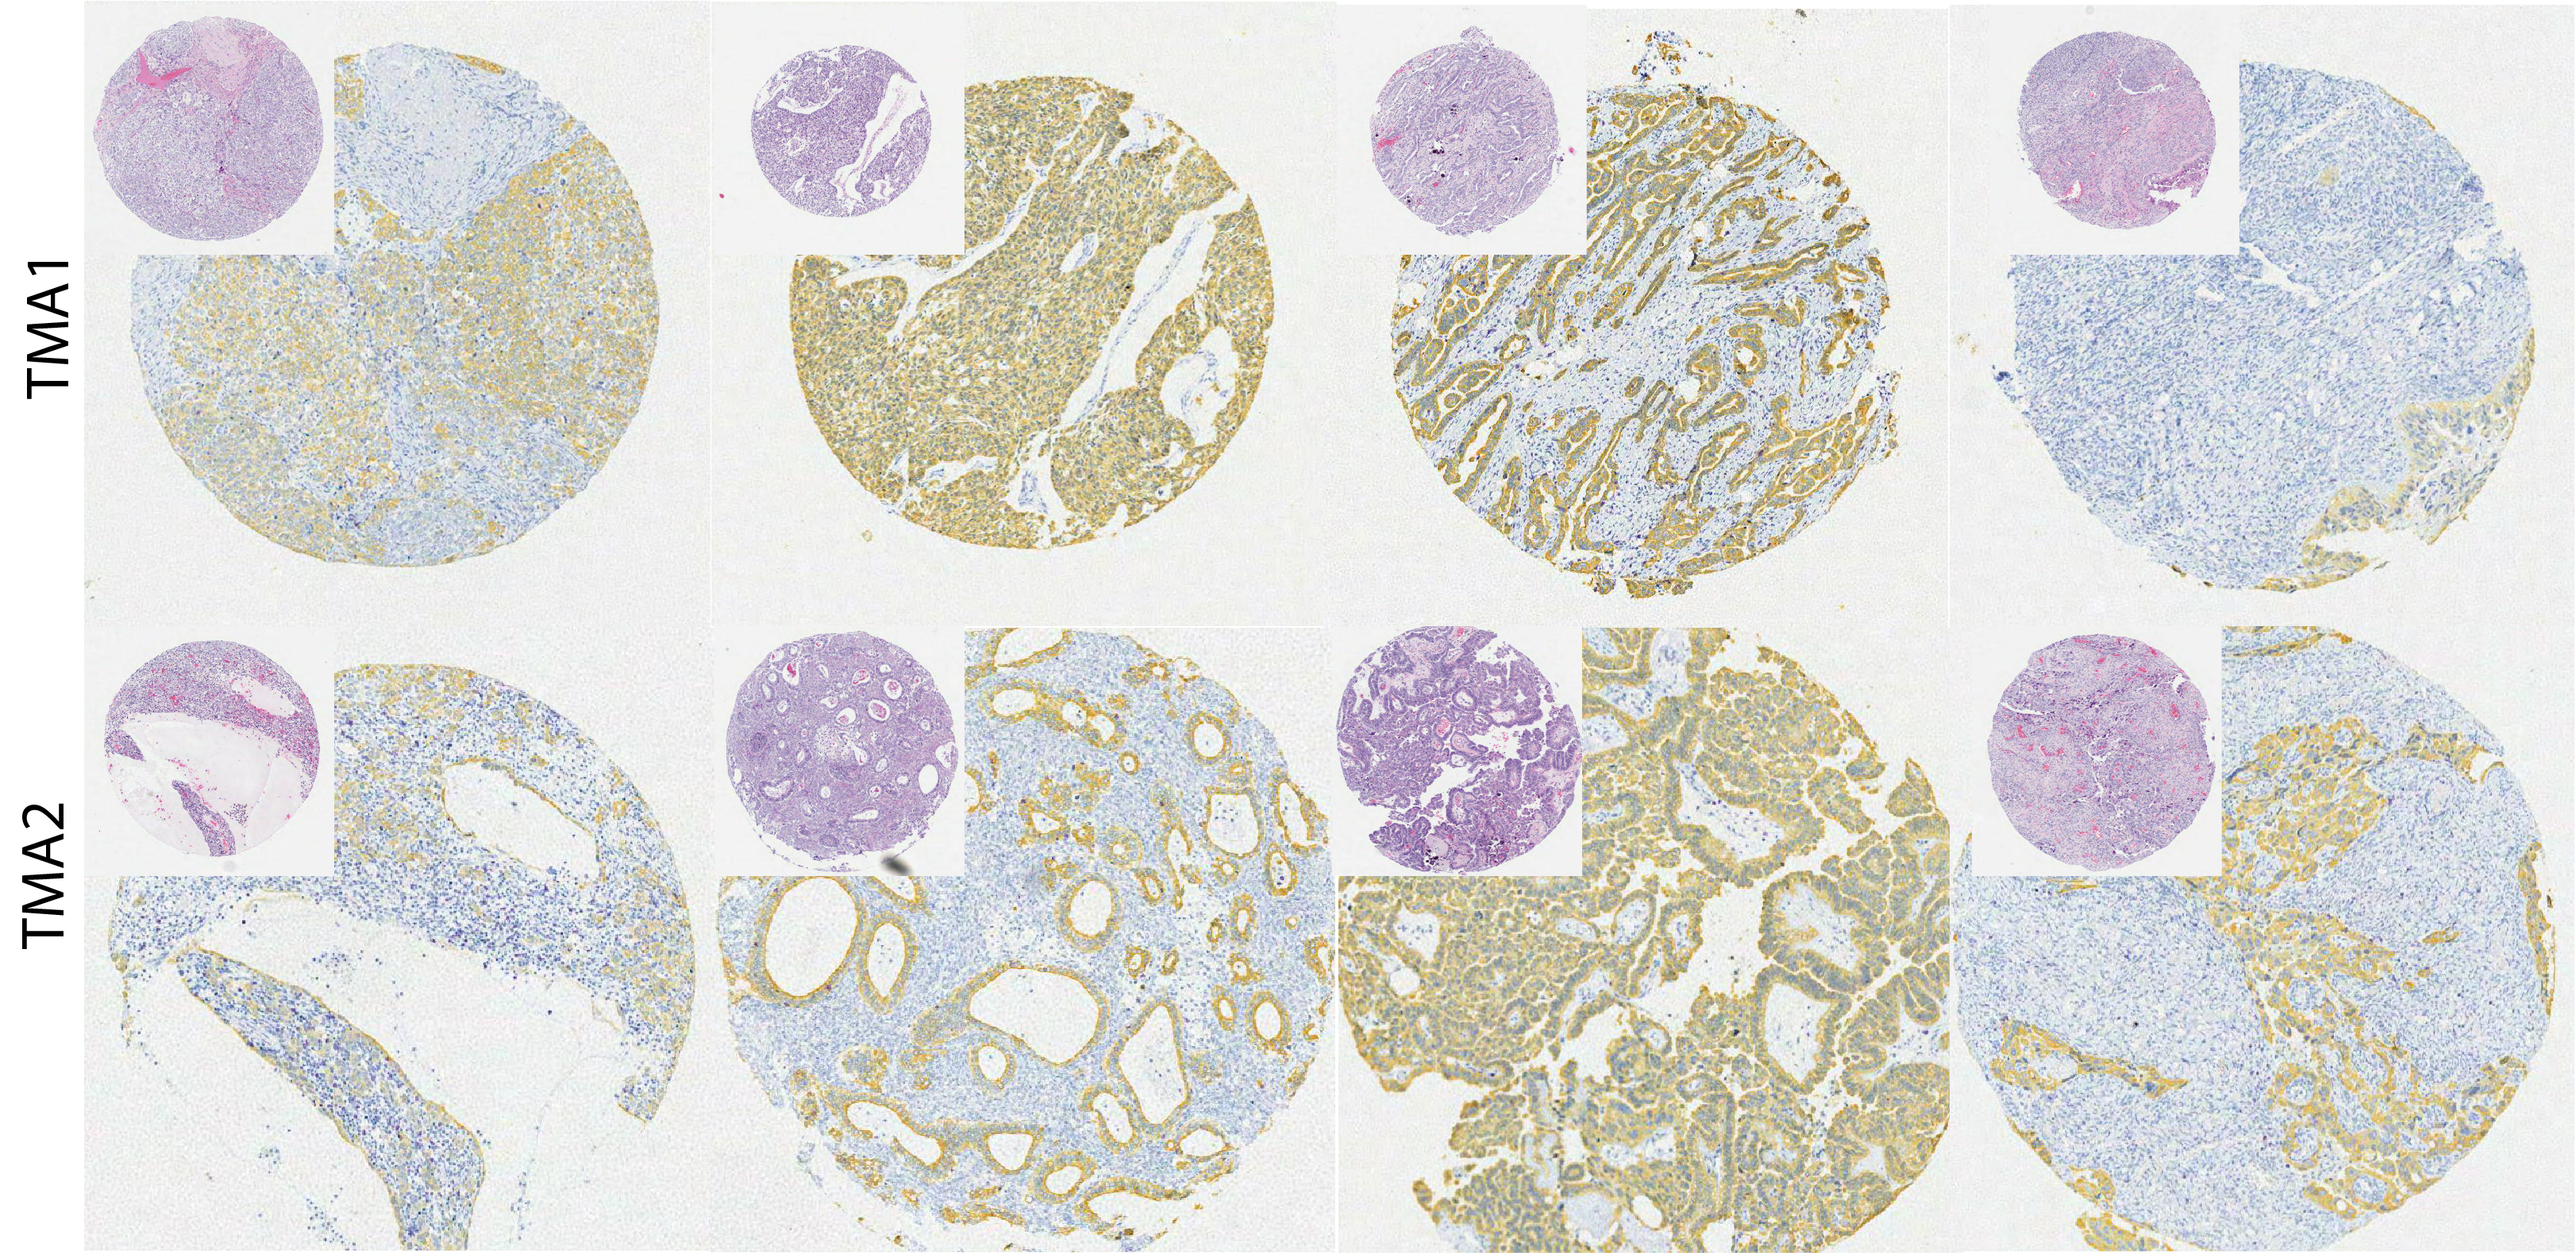
\includegraphics[width=\textwidth]{Chapter3/Figs/Thesis-28.png}
    \caption{Four examples of matched samples that have the most different number of border cells. Top line is TMA1 and bottom line is TMA2. Accompanying serial section H\&E image accompanies each image in the top left to verify no random mispositioning of cores during staining was responsible.}
    \label{fig:outlying_edges}
\end{figure}

\subsubsection{Comparison across different tissue sites}

In order to assess whether this element of tissue structure is conserved across sites of tumours I compared the percent of edge cells in omental vs. ovarian cores. 
\begin{figure}
    \centering
    \includegraphics[width=0.5\textwidth]{Chapter3/Figs/edge_plot_676517_676513.png}
    \caption[Correlation between percentage of epithelial cells classified as border cells for matched Ovarian and Omentum tumour samples]{Correlation between percentage of epithelial cells classified as border cells for matched ovarian and omentum tumour samples from the same patient. Both Pearson and Spearman R and p-value  shown.}
    \label{fig:diff_sites_edge}
\end{figure}

\subsubsection{Comparison with Tumour Grade and Survival}



\subsection{Entropy}
Entropy on some level measures information content and I proposed the use of Entropy measures in order to assess the heterogeneity of samples. The simplest calculation for entropy is the Shannon entropy. In order to utilise this I initially examined entropy as a function of cell types alone and analysed this at multiple scales to examine the tissue features. The formula for deriving entropy is given in Methods \ref{eq:entropy}. I hypothesised that given that tissue regions with mixed cell types would have a higher entropy than those without, that with multiscale area sampling, a reliable classification into tumours with mixing and without could be achieved. 

For each tissue image I calculated the entropy for the whole core, the median across a 4x4 and 10x10.

%Plot increasing jxj median entropy

\subsubsection{Comparing entropy measures across H\&E and CK}
Figure \ref{fig:entropy} gives the mean entropy of the image for serial H\&E and CK stained sections. There was a moderate correlation between these samples. 

\begin{figure}
    \centering
    \includegraphics{Chapter3/Figs/Thesis-06.png}
    \caption{Shannon entropy derived for a H\&E and CK image of serial sections from the same patient core.}
    \label{fig:entropy}
\end{figure}

\subsubsection{Comparing across tissue cores from the same block}
Figure \ref{fig:entropy_block} compares the measures of entropy across tissue samples from the same block but different cores. 
\begin{figure}
    \centering
    \includegraphics{Chapter3/Figs/Thesis____.png}
    \caption{Shannon entropy derived for CK stained images of sections from different cores from the same block. Pearson coefficient was 0.63, $p=1e-10$.}
    \label{fig:entropy_block}
\end{figure}


\subsection{Cell Clustering}

I wanted to understand how cells clustered within a tissue, and to understand the overall composition of the core, is it one solid tissue section or does it have gaps and separations. This can also be understood as whether the tumour and stroma in the core are in multiple parts and whether they are separate or well mixed.

I assessed multiple methods for clustering tissues and in terms of identifying different sizes and shapes of clusters of cells I found that it was best to use DBSCAN, a density based clustering method. An example of a results of another clustering method is shown in Figure \ref{fig:clust_bad}. K-nn clustering, for example, requires a pre-requisite number of clusters, a parameter that varies dramatically between tissue sections. K-nn is also an unsuitable method as when tissue sections comprise varying numbers within groups and varying spatial densities of cells, the method tends to split the cells equally into the pre-specified number of clusters, rather than recognising different sized clusters within.

\begin{figure}
    \centering
    \includegraphics{Chapter3/Figs/knn_example_2.png}
    \caption[k-nearest neighbour clustering of cells]{k-nearest neighbour clustering of cells identified in a tissue section. Densely packed cells are split into pre-specified(n=5) clusters with no biological meaning.}
    \label{fig:clust_bad}
\end{figure}


The DBSCAN method requires two parameters, epsilon (\textit{eps}), the distance within which two points are considered neighbours and \textit{minPts}, the minimum number of points in a cluster.

I decided to only call clusters of at least 15 cells, in tissues making up over 1500 cells, I thought each cluster should contain at least 1\% of the cells in order to improve signal to noise. To derive the optimum \textit{eps} distance for clustering groups of cells on the tissue structure level, I plotted the $k^{th}$ neighbour distribution and located the "elbow" of the curve as discussed in Rahmah et.al. for $k=10$\cite{rahmah2016determination}. The \textit{eps} value obtained from these was 80$\mu$m for Epithelium and 85$\mu$m for Stromal cells. The larger value was used for clustering all cells. These plots for tumour and stroma and the \textit{eps} cutoff from each are shown in Figure \ref{fig:eps}.

\begin{figure}
    \centering
    \includegraphics[width=\textwidth]{Chapter3/Figs/Thesis-11.png}
    \caption{10th nearest neighbour plotted against index, the optimal value for the \texit{eps} is at the elbow of the curve. The \texit{eps} was 80 for All cells, 82 for Tumour and 85 for Stroma.}
    \label{fig:eps}
\end{figure}

An example of DBSCAN clustering on serial H\&E and CK sections is shown in Figure \ref{fig:dbclust}. These show visually accurate identifications of cell clusters across H\&E and CK images. Distributions of the number of stroma, tumour and all cell clusters are shown in figure \ref{fig:dbscatter}.

\begin{figure}
    \centering
    \includegraphics[width=\textwidth]{Chapter3/Figs/dbscan_fullexample.png}
    \caption[DBSCAN example]{Examples of clusters of cells generated with DBSCAN algorithm. Clusters generated from images of tissue sections when epithelial, stromal cells are viewed separately and when all cells are input.}
    \label{fig:dbclust}
\end{figure}

\begin{figure}
    \centering
    \includegraphics{}
    \caption{Number of clusters.}
    \label{fig:dbscatter}
\end{figure}

\subsubsection{Comparison across H\&E and CK}

\subsubsection{Comparison across Tissue Sections}


\subsection{Morphology classification}
Having reliably obtained all the properties above, the quantity of stromal and epithelial cells, identified subclusters, entropy, density of tissue and surface area to volume ratio of the epithelium, I aimed to then investigate whether I could classify tissue sections based upon these features into some of the morphological subtypes mentioned earlier.

I excluded sections which were over 95\% stromal cells, these were classified as stromal and didn't  require further analysis of their structure. 

I decided to select a training set of sections which could easily be classified into the morphologies mentioned by Murakami et. al.  This training set and their labels are shown in \ref{fig:appendix_morphology}.

I compared the metrics measured earlier between these tissue morphologies as shown in Figure \ref{fig:morph_edge}

\begin{figure}
    \centering
    \includegraphics[width=0.8\textwidth]{Chapter3/manual_class_edge_cells.png}
    \caption{Boxplot of the distribution of edge cells for different morphologies.}
    \label{fig:morph_edge}
\end{figure}

Following this decision tree I classified each tissue section as Solid, Papillary Glandular, Desmoplastic/Cribriform or . 

\begin{figure}
    \centering
    \includegraphics{}
    \caption{Histogram of the number of cases classified as solid, glandular, epithelial  or cribriform structure.}
    \label{fig:num_classl}
\end{figure}


\subsection{Relationship between Structure and Immune infiltration}

\subsubsection{Immune quantification}

CD8 and FOXP3 were assessed in OV04 samples.
\begin{itemize}
    \item Correlation between CD8, FOXP3 and edge cells
    \item Immune cells for different structures
\end{itemize}

\subsection{Structure and Survival}

\subsection{Diffusive infiltration model}


\subsection{Collagen structure analysis}
Desmoplasia as mentioned in the previous morphology classification is the formation of fibrous stroma, one dense fibrous stroma component is Collagen. I used Second Harmonic Generation (SHG) to image Collagen on OV04 sections. SHG uses harmonic wave generation by Collagen fibres to image. Figure X shows plot of median collagen entropy and collagen energy for different classifications of tissue.

\subsection{IMC Collagen Analysis?}

\section{Discussion}

Attempts like those of Murakami et. al. \cite{murakami2016establishment} have been made to robustly classify morphologies of HGSOC tissue. Studies have achieved inter-pathologist agreement but automated digital analysis that successfully categorises tissues within HGSOC has not been published. Methods such as deep learning are being attempted but even if successful will not necessarily provide clear insights into the physical features that define the morphologies or a physical understanding of the natural structural variation in samples.

Furthermore, in spite of multiple data sources implying a continuous distribution of densities of infiltration of immune cells into tumours, the literature still dichotimises immune infiltrate and even categorises a subclass of tumour structures as immune reactive, an approach which fails to address the reality that differences in structure may influence immune cells and the rate at which they infiltrate tumours.


In order to address the need for a better structural understanding of tumours before we can relate this to immune infiltration and in order to address the need for automated structural categorisation I generated structural metrics from point patterns of epithelial and stromal cells and examined whether these metrics were correlated across multiple patient samples.

To do this I successfully built classifiers of stroma and epithelium across both Cytokeratin stained and H\&E stained slides. The latter demonstrated that similar methods need not require new staining of sections and could be applied to already available H\&E images that are routinely collected and part of larger public cohorts.

I generated epithelial percentage, border cell, edge cell, entropy based and cluster based metrics and compared them across serial sections stained with H\&E, across sections from cores from the same tissue blocks and across other tumour sites and metastases. I found that the majority of cases were moderately correlated in terms epithelial percentage,  border and edge cells. The most basic method of calculating entropy was not correlated across samples from the same tissue block but the addition of structural information in graphs demonstrated correlation across samples. 




